\documentclass[12pt,twocolumn]{article}
\usepackage[utf8x]{inputenc}
\usepackage[spanish, es-tabla]{babel}
\usepackage{graphicx}

\usepackage{amsmath}

\title{Proyecto Final}
\author{Juan B. Benavides y Juan P. Vanegas }
\date{\today}

\begin{document}
\maketitle

\section{\label{sec: Intro} Sistema Físico}
La entropía es uno de los conceptos físicos más difíciles de comprender. Para llegar a 
él se puede ver desde el punto de vista termodinámico, o desde un punto de vista más 
cercano a la teoría de la información. A partir de este segundo camino podemos definir la 
entropía como 

\section{Algoritmos y Validación}

Para modelar este fenómeno utilizamos dos paradigmas de programación diferentes: Procedimental 
y Orientado a Objetos, cada uno utilizando un algoritmo de propagación diferente. El 
algoritmo utilizado para el paradigma procedimental, descrito en la figura 
\ref{fig:algoritmo_Proc}, que consta en 

\begin{figure}
    \centering
    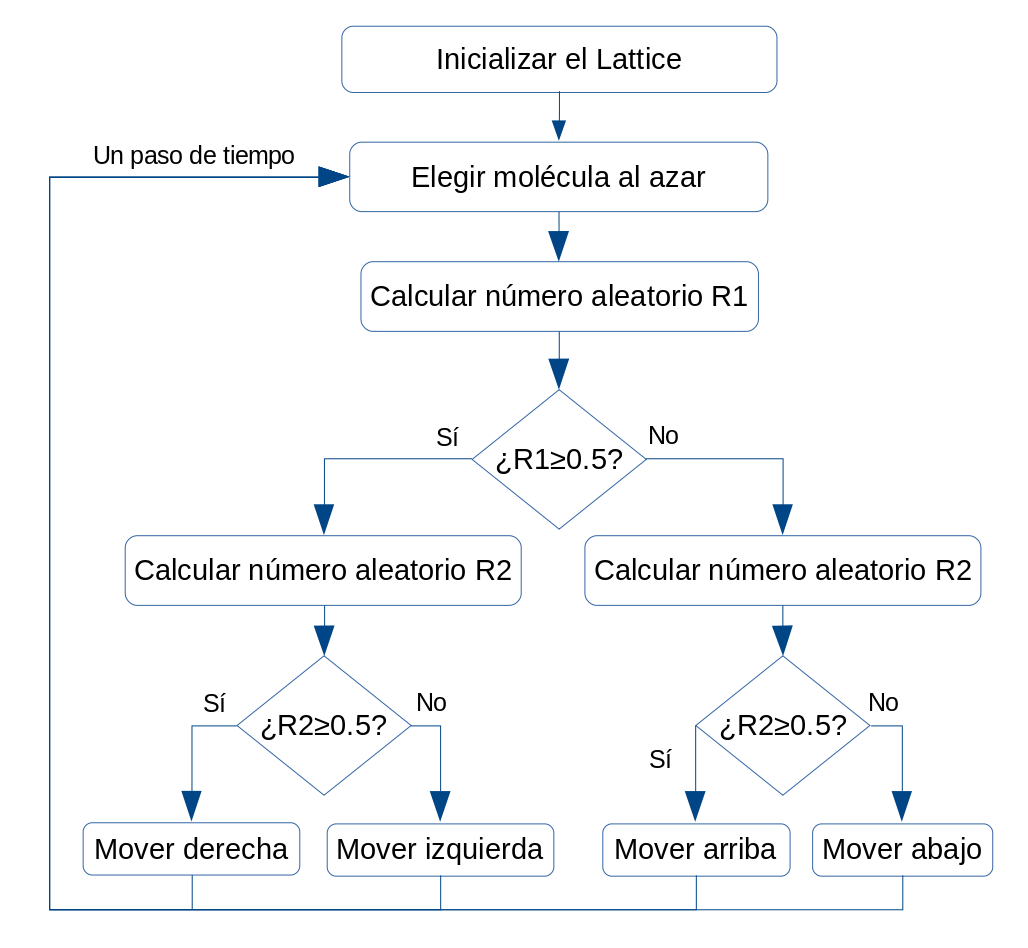
\includegraphics[width=0.3\textwidth]{figs/Algoritmo_Proc.png}
    \caption{Algoritmo 1.}
    \label{fig:algoritmo_Proc}
\end{figure}

Por el otro lado, para el paradigma orientado a objetos se implementó el algoritmo descrito 
en la figura \ref{fig:algoritmo_OOP}, que consiste en una matriz bidimesional de enteros no 
negativos, o Lattice, donde se representan las moléculas como el número de cada celda. Para 
mover las moléculas se recorre el Lattice celda por celda, y en caso de que se encuentre al 
menos una molécula en una celda se mueve a alguna casilla inmediatamente adyacente a la celda. 
Utilizando este algoritmo se toma un paso de tiempo está dado por un recorrido completo al 
Lattice, a diferencia del empleado en el paradigma procedural. 
\\ \\



\begin{figure}
    \centering
    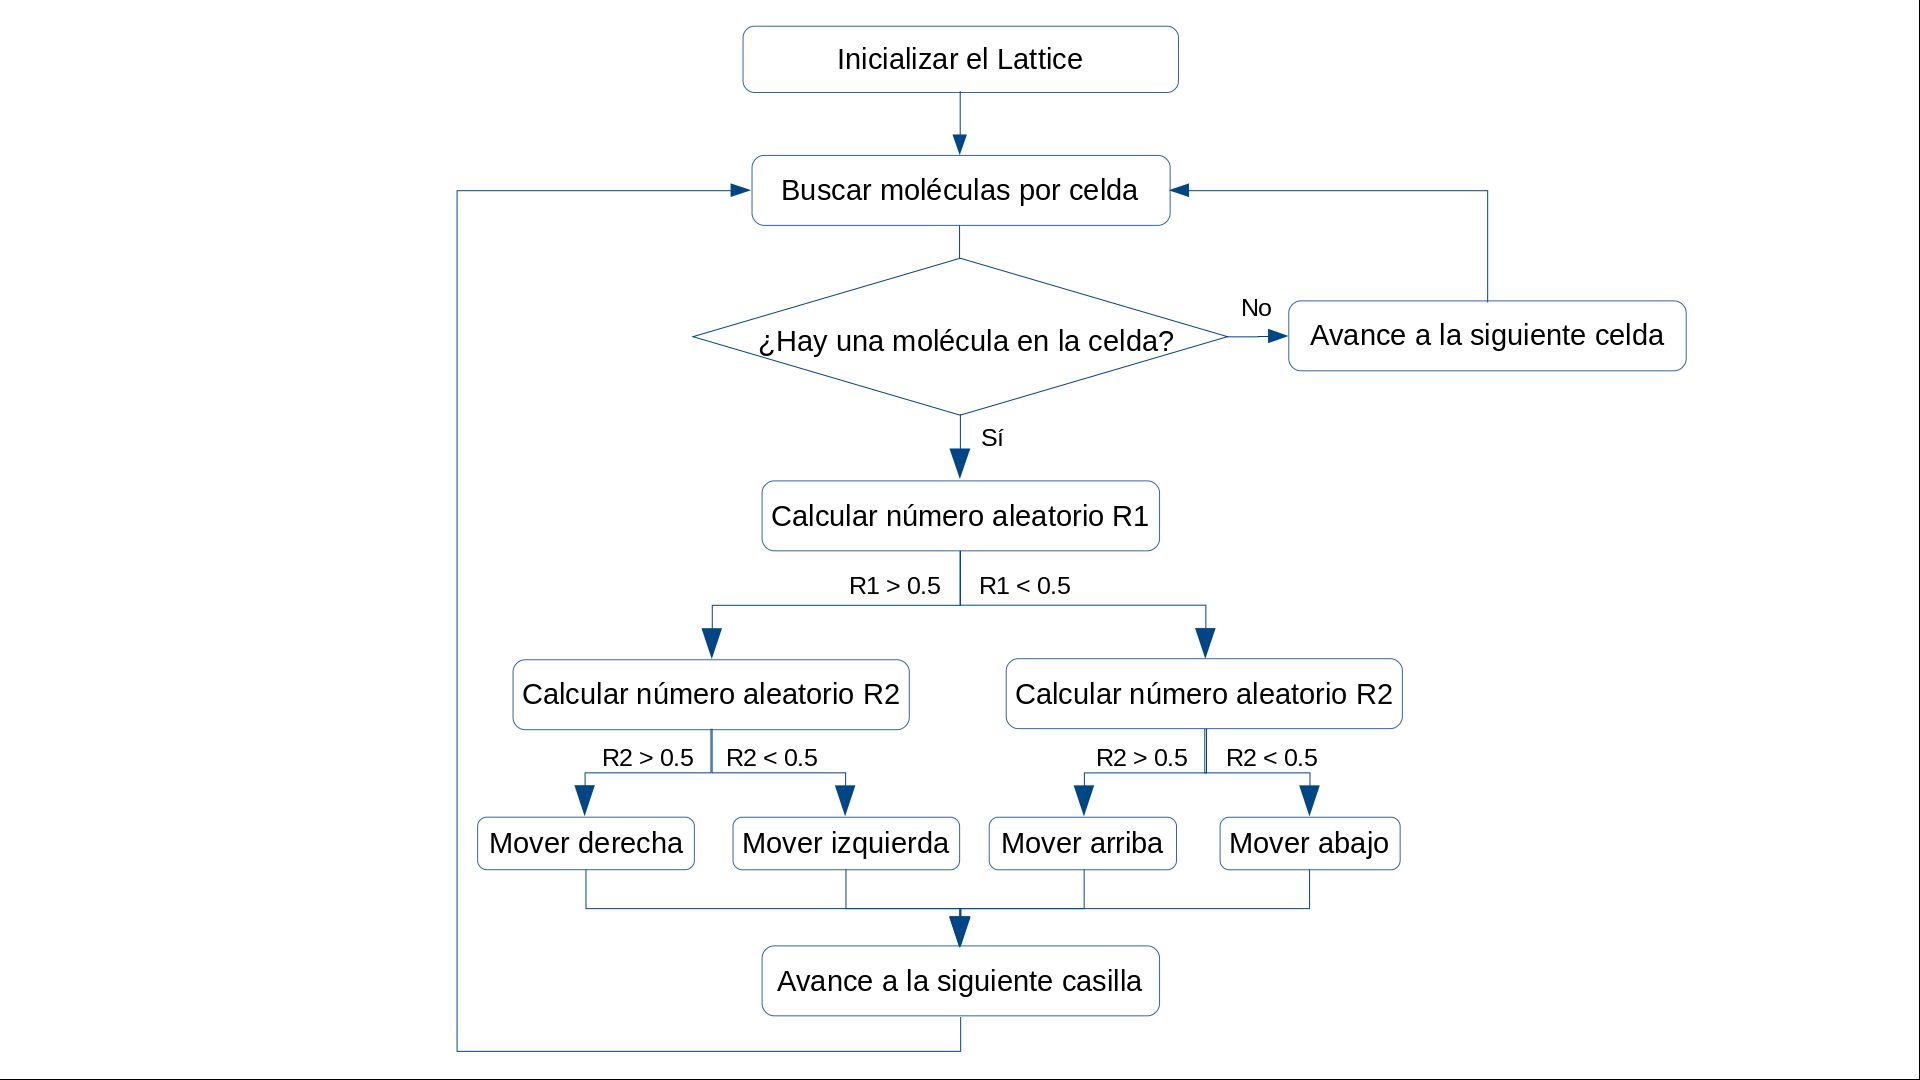
\includegraphics[width=0.3\textwidth]{figs/Algoritmo_OOP.png}
    \caption{Algoritmo 2.}
    \label{fig:algoritmo_OOP}
\end{figure}


\begin{figure}
    \centering
    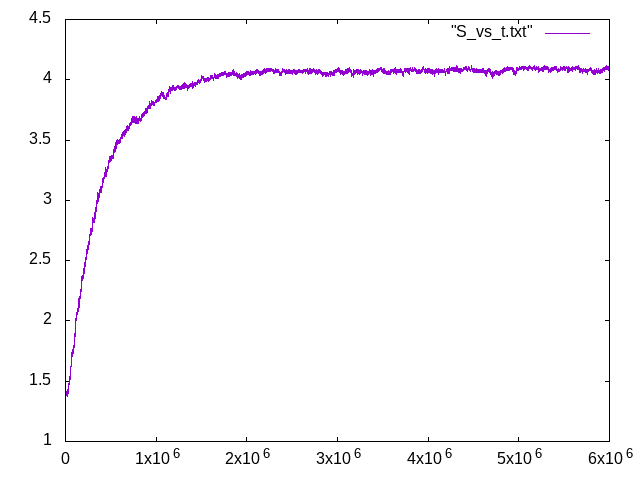
\includegraphics[width=0.3\textwidth]{figs/S_vs_t_OOP_all.png}
    \caption{Entropía en función del tiempo para algoritmo \ref{fig:algoritmo_OOP}.}
    \label{fig:s_vs_t}
\end{figure}

\section{Resultados y Análisis}

\begin{figure}
    \centering
    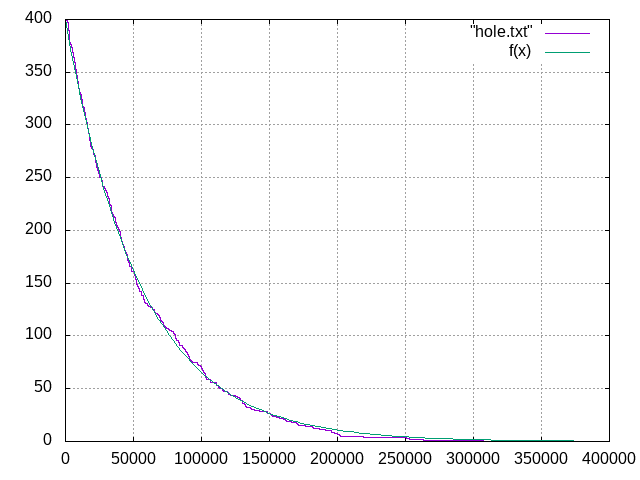
\includegraphics[width=0.3\textwidth]{figs/hole.png}
    \caption{Propagación de las moléculas con un agujero en la pared.}
    \label{fig:hole}
\end{figure}




\section{Conclusiones}

\end{document}